\documentclass[aspectratio=169,11pt]{beamer}
\usepackage[T1]{fontenc}
\usepackage{lmodern,amsmath,amssymb,booktabs,array,graphicx,tikz}
\usetikzlibrary{arrows.meta,positioning,calc}
\definecolor{navy}{HTML}{14334A}
\definecolor{teal}{HTML}{087E8B}
\definecolor{amber}{HTML}{B56317}
\definecolor{rose}{HTML}{AE3150}
\definecolor{muted}{HTML}{536571}
\setbeamercolor{normal text}{fg=navy,bg=white}
\setbeamercolor{structure}{fg=teal}
\setbeamercolor{frametitle}{fg=navy}
\setbeamercolor{alerted text}{fg=rose}
\setbeamercolor{block title}{fg=white,bg=navy}
\setbeamercolor{block body}{fg=navy,bg=navy!5}
\setbeamercolor{block title alerted}{fg=white,bg=rose}
\setbeamercolor{block body alerted}{fg=navy,bg=rose!5}
\setbeamertemplate{navigation symbols}{}
\setbeamertemplate{itemize items}[circle]
\setbeamersize{text margin left=8mm,text margin right=8mm}
\setbeamerfont{frametitle}{size=\Large,series=\bfseries}
\setbeamertemplate{frametitle}{\vspace{3mm}\insertframetitle\par\vspace{1mm}{\color{teal}\rule{\linewidth}{.65pt}}}
\setbeamertemplate{footline}{\hspace{8mm}\textcolor{muted}{\scriptsize NPS $\pi^0$\enspace /\enspace KinC\_x60\_4b LH$_2$\enspace /\enspace diagnostic study}\hfill\textcolor{muted}{\scriptsize\insertframenumber}\hspace{8mm}\vspace{3mm}}
\hypersetup{colorlinks=true,urlcolor=teal,pdftitle={NPS livetimes: definitions, evidence and KinC x60 4b LH2},pdfauthor={NPS pi0 analysis working notes}}
\newcommand{\source}[1]{\par\vfill{\scriptsize\color{muted}#1\par}}
\newcommand{\takeaway}[1]{\begin{beamercolorbox}[sep=2.5mm,wd=\linewidth]{block body}\textbf{#1}\end{beamercolorbox}}
\newcommand{\plotframe}[3]{\begin{frame}{#1}\centering\includegraphics[width=\linewidth,height=.59\textheight,keepaspectratio]{figures/#2.pdf}\par\vspace{1mm}\raggedright\small #3\end{frame}}
\newcommand{\Lp}{\widehat L_{\rm EDTM}}
\newcommand{\Lphys}{\widehat L_{\rm phys}}
\newcommand{\Lall}{\widehat L_{\rm all}}
\newcommand{\LLone}{\widehat L_{\rm L1}}
\title{What does our livetime actually measure?}
\subtitle{Definitions, matched counters, and artificial normalization structure\\KinC\_x60\_4b\enspace LH$_2$}
\author{NPS $\pi^0$ analysis\quad Working technical presentation}
\date{9 September 2026\quad Frozen cache results + source investigation}
\begin{document}
\begin{frame}[plain]
\vspace{8mm}{\color{teal}\large NPS\quad /\quad NORMALIZATION STUDIES}\par\vspace{7mm}
{\LARGE\bfseries\inserttitle\par}\vspace{4mm}{\large\insertsubtitle\par}\vspace{6mm}
\takeaway{A plausible ratio is only useful when its population, coverage, and signal path are known.}
\vfill\small\insertauthor\par\insertdate\par\vspace{2mm}
\scriptsize Numerical baseline: 168 cached segments, before the new staging completes.\\
Diagnostic results; no production correction has been replaced.
\end{frame}

\begin{frame}{Three questions organize the investigation}
\begin{enumerate}\setlength\itemsep{5mm}
\item \textbf{What loss can each counter see?}\\Electronic, TI/DAQ, recorded-event and pulser populations differ.
\item \textbf{Are numerator and denominator counting the same exposure?}\\Initial baselines, terminal snapshots, beam trips and segment gaps matter.
\item \textbf{Would using this ratio distort a physics result?}\\Prescales, timing acceptance and rate weighting remain conditions to test.
\end{enumerate}
\source{Main discussion: definitions, prior attempts, methodology and comparisons. Backup: exact counts, variants, source provenance and reproduction.}
\end{frame}

\begin{frame}{Name the stages before naming the livetimes}
\centering
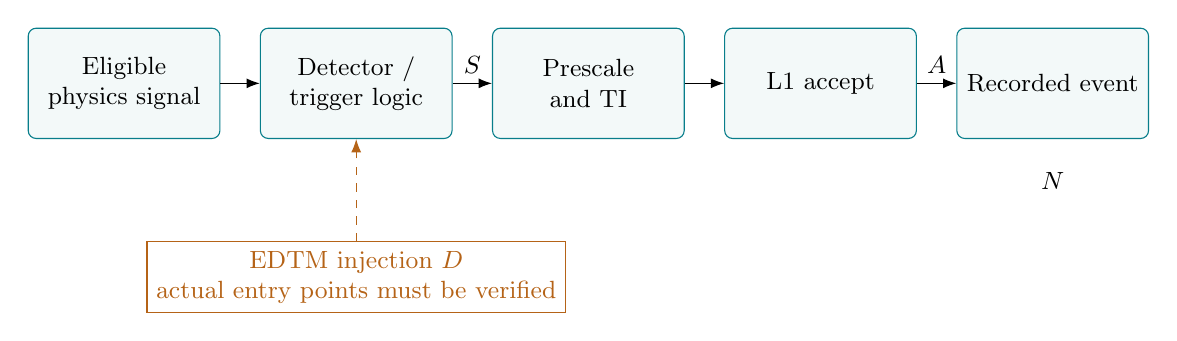
\begin{tikzpicture}[>=Latex,node distance=5mm,box/.style={draw=teal,fill=teal!5,rounded corners=1mm,minimum height=14mm,text width=22mm,align=center,font=\small}]
\node[box] (ideal) {Eligible physics signal};
\node[box,right=of ideal] (logic) {Detector / trigger logic};
\node[box,right=of logic] (ps) {Prescale and TI};
\node[box,right=of ps] (l1) {L1 accept};
\node[box,right=of l1] (rec) {Recorded event};
\draw[->] (ideal)--(logic);\draw[->] (logic)--node[above,font=\small]{$S$}(ps);\draw[->](ps)--(l1);\draw[->](l1)--node[above,font=\small]{$A$}(rec);
\node[below=3mm of rec,font=\small] {$N$};
\node[below=13mm of logic,draw=amber,text=amber,align=center,font=\small] (edtm) {EDTM injection $D$\\actual entry points must be verified};
\draw[->,amber,dashed](edtm)--(logic);
\end{tikzpicture}
\vspace{4mm}
\takeaway{EDTM samples the path downstream of its injection points. It does not automatically test every detector or NPS trigger loss.}
\source{Conceptual stage diagram, not a certified run-period wiring diagram. $S$ is the selected input tap, $A$ the L1 tap; $E\subset N$ is recorded EDTM.}
\end{frame}

\begin{frame}{Electronic, DAQ and total livetime: conditional definitions}
\small
Let $G$ be a signal satisfying fixed detector/trigger criteria absent rate losses; $B$ formation of that input; $P$ passing the prescale; $R$ recording it.
\begin{align*}
L_{\rm elec}&=\Pr(B\mid G) &&\text{loss before the input tap},\\
L_{\rm DAQ}&=\Pr(R\mid P,B,G) &&\text{loss after prescale eligibility},\\
\Pr(R\mid G)&=L_{\rm elec}\,\Pr(P\mid B,G)\,L_{\rm DAQ}.
\end{align*}
\takeaway{For representative prescaling, $\Pr(P\mid B,G)=1/p$ and $L_{\rm total}\equiv p\Pr(R\mid G)=L_{\rm elec}L_{\rm DAQ}$.}
\vspace{2mm}
\small The product is a conditional-probability chain, not an assumption that losses are independent. Trigger thresholds, offline tracking/PID efficiencies and data-quality cuts require their own defined reference populations.
\source{Operational definitions for this talk. ``Computer LT'' is often used for several different tap-to-tap ratios; always supply the actual formula. Historical terminology: Pooser, DocDB 1022.}
\end{frame}

\begin{frame}{Time sampling and physics-event sampling can differ}
\begin{columns}[T]
\column{.49\textwidth}
\textbf{Time-weighted availability}
\[L_{t}=\frac{1}{T}\int a(t)\,dt\]
Uniform pulser times approximate this only if their phase and acceptance sample the system representatively.
\column{.49\textwidth}
\textbf{Physics-rate-weighted availability}
\[L_r=\frac{\int r(t)a(t)\,dt}{\int r(t)\,dt}\]
High-rate periods contribute more physics events and can have lower availability.
\end{columns}
\vspace{4mm}
\takeaway{The same current cut helps match exposure; it does not prove identical weighting.}
\source{$a(t)$: availability; $r(t)$: eligible input rate. For stable yield per charge, the relevant effective factor is $L_Q=\int I(t)L(t)dt/\int I(t)dt$. Current intervals here are averages; good-helicity/yield/charge matching is still pending.}
\end{frame}

\begin{frame}{Five counts and one prescale define the diagnostic ratios}
\begin{columns}[T]
\column{.50\textwidth}\small
\begin{tabular}{@{}cl@{}}\toprule
$N$ & Recorded events\\
$E$ & Accepted EDTM subset of $N$\\
$S$ & Selected trigger input scaler\\
$D$ & Sent EDTM scaler\\
$A$ & L1 accept scaler\\
$p$ & Intentional prescale factor\\\bottomrule
\end{tabular}
\vspace{4mm}\par All counts refer to the \textbf{same selected intervals}.
\column{.47\textwidth}
\begin{align*}
\Lp&=pE/D\\
\Lall&=pN/S\\
\Lphys&=p(N-E)/(S-D)\\
\LLone&=pA/S
\end{align*}
\end{columns}
\source{Hats emphasize estimators. Subtraction requires one pulser contribution per chosen input, valid EDTM classification and a common representative prescale. $S-D$ must be positive. $N/A$ is a separate recorded-versus-L1 closure check.}
\end{frame}

\begin{frame}{Accepted pulses and sent pulses belong on different sides}
\small
\[\Lphys=\frac{p\,\underbrace{(N-E)}_{\text{recorded physics}}}{\underbrace{(S-D)}_{\text{input physics}}}\]
\begin{itemize}\setlength\itemsep{2mm}
\item Removing $D$ from the accepted count subtracts pulses that may never have been recorded.
\item At $p=1$, replacing $N-E$ by $A-D$ is equivalent only if $N=A$ and $E=D$.
\item These ratios share counts and satisfy an exact identity:
\end{itemize}
\[\boxed{\Lall=\left(1-\frac{D}{S}\right)\Lphys+\frac{D}{S}\Lp}\]
\source{Agreement among these ratios is useful closure, not three independent measurements of total livetime. Multiplying overlapping EDTM and DAQ factors would count some losses twice.}
\end{frame}

\begin{frame}{The cache baseline covers every production run, partially in places}
\small
\begin{columns}[T]
\column{.49\textwidth}
{\Huge\color{teal}43}\par\textbf{production runs represented}\par\vspace{4mm}
46 cached runs in total; 168 selected segments; 70,155,126 recorded events.
\column{.49\textwidth}
\textbf{51 LH$_2$ metadata entries}\par
43 production, 6 junk, 2 efficiency. Five junk entries had no selected cache files.
\vspace{4mm}\par Updated replay preferred per run; production replay used as fallback. Alternate replays are not independent segments.
\end{columns}
\vspace{2mm}\takeaway{All runs represented does not mean all segments available. New staging requires a fresh manifest and calculation.}
\source{Frozen inventory: 2026-09-09 18:56 UTC. 253 candidate files included 85 alternate replay files. Numeric figures retain that snapshot; cache availability is recorded separately. No jcache invoked.}
\end{frame}

\begin{frame}{What we tried before: the May 2025 luminosity study}
\small\renewcommand{\arraystretch}{1.35}
\begin{tabular}{@{}p{.23\textwidth}p{.32\textwidth}p{.39\textwidth}@{}}\toprule
Method & Population used & Why it did not settle this problem\\\midrule
Total EDTM & Whole-file accepted / sent; no current cut on definition slide & Event tails and initial scaler counts need not describe the same exposure.\\
Computer LT, TSH & Beam-on L1 / trigger scalers & Only losses between taps; depends on valid scaler increments.\\
Computer LT, TDC & Whole-file TDC count scaled by beam-on fraction & A fraction is a proxy, not direct event/interval assignment.\\
Physics CLT, TDC & Remove EDTM; apply beam-on proxy & Same coverage issue plus accepted/sent and routing assumptions.\\\bottomrule
\end{tabular}
\source{Singh, May 2025 NPS luminosity presentation, especially slide 23; archived code inspected. Historical problems in runs 1526--1534 are not established causes for KinC\_x60\_4b.}
\end{frame}

\begin{frame}{Current NewGen: preserve the actual applied reference}
\begin{columns}[T]
\column{.53\textwidth}\small
\textbf{Numerator:} $T$-stored current; finite raw EDTM $>1$; within $\pm500$ raw channels of the run peak.
\vspace{3mm}\par\textbf{Denominator:} consecutive TSH differences per file; ending-row current within the helper window.
\vspace{3mm}\par\textbf{Helper:} per-segment TSHelH current peak, 0.5-$\mu$A bins, $\pm15\%$ window.
\column{.44\textwidth}
\includegraphics[width=\linewidth,height=.54\textheight,keepaspectratio]{figures/applied_NewGen.png}
\scriptsize Original user-supplied figure, unchanged. Numeric comparisons use its saved CSV.
\end{columns}
\source{42 production runs with the same saved coverage reproduce $E,D$ and raw peak exactly. Run 4398 changed from one to six cached segments. $500$ raw channels $\simeq48.83$ ns; the source comment saying ``500 ns'' is incorrect.}
\end{frame}

\begin{frame}{Run 4398 exposes the endpoint mismatch directly}
\begin{columns}[T]
\column{.49\textwidth}
\textbf{Segment 0: current NewGen}
\[\frac{19341}{19310}=1.00160539\]
Last real boundary: event 541321.\\
Terminal row: 542585, unchanged clock and primary counters.
\column{.49\textwidth}
\textbf{Restrict to measured coverage}
\[\frac{19292}{19310}=0.99906784\]
1264 uncovered tail events include \textbf{49 raw-window EDTM candidates}.
\end{columns}
\vspace{4mm}\takeaway{Changing a denominator formula cannot supply a missing final scaler interval.}
\source{Same current selection; raw-window comparison isolates the coverage effect. Tight timing gives $19290/19310=0.99896427$. Initial scaler values include 878 pulser and 23020 TRIG4 counts before the first recorded boundary; treat them as a baseline.}
\end{frame}

\begin{frame}{New calculation: one explicit interval for every count}
\centering
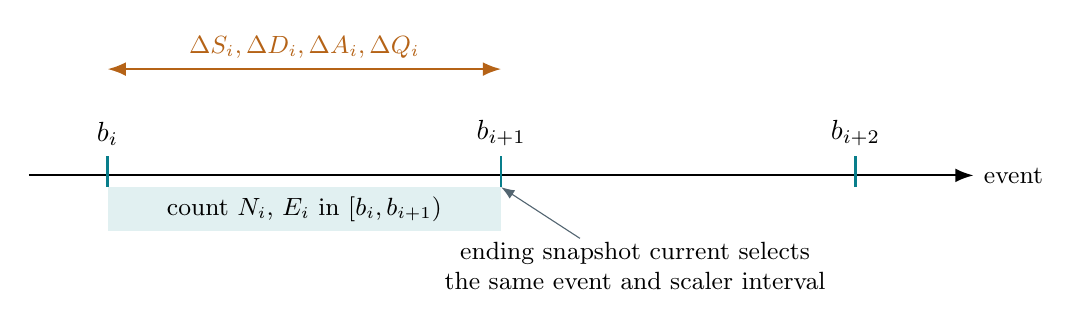
\begin{tikzpicture}[>=Latex,x=1cm,y=1cm]
\draw[->,thick] (0,0)--(12,0) node[right,font=\small]{event};
\foreach \x/\b in {1/{b_i},6/{b_{i+1}},10.5/{b_{i+2}}}{\draw[teal,thick](\x,-.15)--(\x,.25);\node[above]at(\x,.25){$\b$};}
\fill[teal!12](1,-.7)rectangle(6,-.15);
\node[font=\small]at(3.5,-.43){count $N_i$, $E_i$ in $[b_i,b_{i+1})$};
\draw[<->,amber,thick](1,1.35)--node[above,font=\small]{$\Delta S_i,\Delta D_i,\Delta A_i,\Delta Q_i$}(6,1.35);
\node[align=center,font=\small]at(7.7,-1.15){ending snapshot current selects\\the same event and scaler interval};
\draw[->,muted](7,-.8)--(6,-.15);
\end{tikzpicture}
\vspace{2mm}
\[\Lp=p\,\frac{\sum_{i\in\mathcal G}E_i}{\sum_{i\in\mathcal G}\Delta D_i}\qquad
\Lphys=p\,\frac{\sum_{i\in\mathcal G}(N_i-E_i)}{\sum_{i\in\mathcal G}(\Delta S_i-\Delta D_i)}\]
\source{$b_i=\mathrm{TSH.evNumber}$; event coordinate is $T$'s \texttt{g.evnum}. $\mathcal G$ is the common current-selected coverage. Sum counts before dividing. Alternate $(b_i,b_{i+1}]$ tests the unresolved single-event latch convention.}
\end{frame}

\begin{frame}{Files are storage boundaries; gaps are exposure boundaries}
\begin{enumerate}\setlength\itemsep{3mm}
\item Join adjacent segments only with event continuity and compatible monotonic clock, trigger, EDTM, L1 and charge counters.
\item Split at missing segments or restarts; exclude uncovered heads/tails. The first cumulative values are a baseline.
\item Remove a snapshot as duplicate only when its clock \textbf{and all primary counters} are unchanged.
\end{enumerate}
\vspace{2mm}\takeaway{Zero elapsed clock with changing counters is an anomaly, not an ordinary duplicate.}
\source{Internal negative increments stop a run for investigation. Counter anomalies remain in the audit. Ending-file current window is used across a compatible file boundary. A neighboring file can recover a preceding file's uncovered tail.}
\end{frame}

\begin{frame}{A tighter timing window is a sensitivity test}
\begin{columns}[T]
\column{.49\textwidth}\textbf{Computed diagnostic}
\small\par Run-specific corrected-time peak: 0.1-ns mode, then median within 1 ns. Require raw time $>1$ and corrected time within $\pm2$ ns.
\vspace{3mm}\par Compare raw-window counts and half-widths 0.5, 1, 2, 3, 5, 10, 20, 50 ns.
\column{.49\textwidth}\textbf{New literature caveat}
\small\par Murphy's PionLT study reports valid EDTM outside the corrected-time peak. Its trigger configuration differs from NPS.
\vspace{3mm}\par Peak purity and pulse acceptance are separate questions. Raw/reference timing and multiple-hit information must identify the rejected candidates.
\end{columns}
\vspace{3mm}\takeaway{Do not label the $\pm2$ ns estimate as a certified total livetime or call every rejected tail event noise.}
\source{Murphy, \href{https://redmine.jlab.org/attachments/download/1499/EDTM_Study_Report.pdf}{EDTM Study Report}, 28 June 2022, sections 1--3. Applicability warning, not proof of NPS signal loss.}
\end{frame}

\plotframe{All production runs: retain the saved and same-cache controls}{comparison_all}{Orange open: saved NewGen; orange crosses: recomputed on the diagnostic cache. Blue: matched $\pm2$ ns EDTM; green: conditional physics CLT. Shading marks prescales; red rings mark counter defects. No clipping.}
\plotframe{Unprescaled runs reveal structure hidden by the large excess}{comparison_unprescaled}{This view changes only the plotted subset. Counter defects remain; proximity to unity is not an acceptance test. All ratios use the frozen cache snapshot.}
\plotframe{Changing the method has several distinct contributions}{decomposition}{These are sequential, order-dependent changes on identical files, in percentage points. Coverage and interval-current assignment are separate from joining files and changing timing.}

\begin{frame}{Run 4398: method changes and file changes must be separated}
\small\renewcommand{\arraystretch}{1.35}
\begin{tabular}{@{}p{.49\textwidth}rr@{}}\toprule
Calculation & Segments & Ratio\\\midrule
Saved applied NewGen & 1 & 1.00160539\\
NewGen on diagnostic cache & 6 & 0.99858088\\
Matched $\pm2$ ns EDTM & 6 & 0.99914853\\
Matched physics CLT (conditional) & 6 & 0.99916851\\\bottomrule
\end{tabular}
\vspace{4mm}\takeaway{The saved-to-new difference combines coverage and method. The same-cache control isolates the method comparison.}
\source{Matched counts: $N=A=2893284$, $S=2895694$, $D=112746$, $E_{\rm raw}=112658$, $E_{\pm2}=112650$. Current: 33.3625--45.1375 $\mu$A. Full cache includes 3,222,394 events before interval/current selection.}
\end{frame}

\plotframe{Prescaled runs require a sampling check of their own}{prescales}{For run 4259, $p=5$: $pE/D=1.03042$, while $pN/S=0.999253$ and $p(N-E)/(S-D)=0.995225$. $E/D<1$; the corrected ratio above one is not literally more accepted than sent pulses.}

\begin{frame}{A prescale factor is not enough to establish pulser sampling}
\begin{itemize}\setlength\itemsep{3mm}
\item Metadata selects one enabled trigger per run. Setting 0 means $p=1$; otherwise $p=2^{s-1}+1$. Thus setting 1 gives 2; setting 3 gives 5.
\item Periodic pulses can correlate with prescale state or busy timing. Multiple enabled triggers add acceptance competition and timing priority.
\item All recorded events carry the configured trigger bit. This checks the replay population; it does not independently establish run-start routing or TI mode.
\end{itemize}
\source{40 populated Run\_Data prescale records agree with metadata; 128 all-zero records are placeholders, and all set/read flags are zero. Murphy section 4 illustrates trigger competition in PionLT; it does not establish the cause of run 4259's residual.}
\end{frame}

\begin{frame}{A ratio near one can hide inconsistent counters}
\small\renewcommand{\arraystretch}{1.3}
\begin{tabular}{rrrrrrr}\toprule
Run & $\Delta t$ (s) & $N$ & $A$ & $S$ & $D$ & $E$\\\midrule
4303 & 0.000869 & 1915 & 3 & 3 & 1 & 79\\
4305 & 0.005481 & 1047 & 2 & 2 & 0 & 80\\\bottomrule
\end{tabular}
\vspace{4mm}
\begin{itemize}\setlength\itemsep{2mm}
\item These selected intervals violate recorded-versus-L1 closure far beyond a one-event latch ambiguity.
\item Run 4303's aggregate EDTM ratio is still $0.999782$.
\item Exclusion variants are tabulated, \textbf{not adopted}. If excluded later, yield and charge must lose the same exposure.
\end{itemize}
\source{Diagnostic flag: $N-A>4$, above ordinary one/two-count latch differences. Independent ROOT/uproot reads verify representative stored values and the run 4305 mismatch; they do not identify the raw DAQ cause.}
\end{frame}

\plotframe{Real DAQ losses must remain in the livetime}{intervals_4398}{At about 820.126 s: $S=2082$, $N=A=1799$, $D=80$, $E=69$ over roughly 2 s. Both event and L1 counts show the loss. This is not the same signature as $N\gg A$; do not remove it to flatten a plot.}

\begin{frame}{PRE40/100/150/200: populated does not mean identified}
\begin{columns}[T]
\column{.49\textwidth}\textbf{Established from the replay map}
\small\par ROC 5: hPRE100 / hPRE150 at slot 10 channels 9 / 10. The branches hold counts.
\vspace{3mm}\par Run 4398 segment 0: hPRE150/hPRE100 $=0.9906772$; p-side ratio $=0.9554787$.
\column{.49\textwidth}\textbf{Still required for a correction}
\small\par Input trigger and run-period cabling; actual widths and module modes; gating; relation to physics trigger logic and EDTM injection.
\vspace{3mm}\par Rate correlation with a TRIG channel is a candidate lead, not wiring proof.
\end{columns}
\vspace{3mm}\takeaway{No PRE-derived correction is applied. In particular, the p-prefix cannot be treated as proof that a monitor measures NPS deadtime.}
\source{Run-4398 archived map and measurements. The Hall C trigger-history page links a 16 February 2018 cabling entry (3532998); its existence does not establish February 2024 wiring. PRE model assumptions are in backup.}
\end{frame}

\begin{frame}{New NPS sources sharpen the questions we can ask}
\small
\begin{columns}[T]
\column{.49\textwidth}\textbf{Zhang, July 2024}
\small\par Discusses timing noise, anomalous scaler behavior and report-file LT discrepancies. NPS-side loss remains a separate question.
\vspace{3mm}\par Earlier March work used raw-time cuts, a 2-$\mu$A cut, inferred scaler repairs and terminal-readout removal.
\column{.49\textwidth}\textbf{Raydo, July 2024}
\small\par Trigger and waveform-readout thresholds differ. FADC/VTP configurations are stored in beginning-of-run EVIO and uploaded to the logbook.
\vspace{3mm}\par Recovering these records is a concrete route to run-specific configuration evidence.
\end{columns}
\source{\href{https://indico.jlab.org/event/866/contributions/14918/subcontributions/283/attachments/11529/17843/Deadtime\%20and\%20Efficiency.pdf}{Zhang, 18 July 2024}, slides 5--13; \href{https://redmine.jlab.org/attachments/download/2368/Updates_2024-03-03.pdf}{3 March 2024}, slide 1; \href{https://indico.jlab.org/event/866/contributions/14914/subcontributions/234/attachments/11505/17805/NPS_July17_2024_Raydo.pdf}{Raydo, 17 July 2024}, slides 2, 7--8. Not run-start records themselves.}
\end{frame}

\plotframe{Normalization errors can introduce artificial run structure}{normalization_effect}{For fixed yield and charge, changing only $L$ gives $Y_{\rm new}/Y_{\rm old}-1=L_{\rm old}/L_{\rm new}-1$: $-0.76662\%$ (4493) to $+0.69710\%$ (4308). This is a conditional illustration, not a measured cross-section bias.}

\begin{frame}{The physics risk is more than a common scale shift}
\[Y_b=\sum_{r}\frac{n_{rb}}{Q_r\,L_r\,\epsilon_r}\quad\text{(schematic normalization)}\]
\begin{itemize}\setlength\itemsep{3mm}
\item A common fractional LT error changes normalization. A run-dependent error can change a bin's shape when its run mixture differs.
\item Current/rate dependence can imitate yield slopes; helicity-dependent coverage can contaminate an asymmetry.
\item A flat yield is a cross-check after defining the correction, not a rule for choosing it. LH$_2$ density and other efficiencies can also vary.
\end{itemize}
\source{The schematic is not a claim about the production combination formula. Prescale weighting, efficiencies, charge and selected exposure must follow that formula consistently. No physics yields or production correction files were changed here.}
\end{frame}

\begin{frame}{What is established, and what must still be tested}
\small
\begin{columns}[T]
\column{.49\textwidth}\textbf{Established in the cached replays}
\small\begin{itemize}\setlength\itemsep{2mm}
\item NewGen count reproduction.
\item Endpoint/current mismatch and explicit common-interval calculation.
\item Prescaled residuals, counter defects and real loss bursts.
\end{itemize}
\column{.49\textwidth}\textbf{Before choosing a production prescription}
\small\begin{itemize}\setlength\itemsep{2mm}
\item EDTM timing acceptance and representative sampling.
\item PRE routing, TI mode, run-start configuration and counter cause.
\item Full staged coverage, good-helicity/yield/charge matching and uncertainty model.
\end{itemize}
\end{columns}
\vspace{1mm}\takeaway{Match the counts, identify the path, preserve genuine losses, and carry unresolved effects into the interpretation.}
\source{All figures remain diagnostic. The next cache calculation must freeze its own selected replay manifest and retain both same-cache method controls and old-snapshot comparisons.}
\end{frame}

\appendix
\begin{frame}{Backup: exact methodology, counter evidence and sources}
\large Reference material for technical questions\par\vspace{5mm}
\normalsize Timing and latch variants; individual counter diagnostics; historical estimators; PRE assumptions; uncertainty; all-production numeric tables; reproducibility.
\source{Editable LaTeX text and equations; native TikZ diagrams; vector PDF analysis figures. Original frozen numerical archive is preserved separately.}
\end{frame}

\plotframe{Production comparison: runs 4253--4397}{comparison_early}{Same legend and diagnostic conditions as the main comparison. The run-number spacing is compressed to ordered positions. The saved reference and same-cache NewGen are separate series.}
\plotframe{Production comparison: runs 4398--4558}{comparison_late}{Run 4398's saved reference used one segment. Six segments enter its same-cache comparison. The other saved production count pairs reproduce exactly where file coverage is unchanged.}
\plotframe{Timing spectra and timing acceptance need separate checks}{timing_sensitivity}{The corrected-time peak is narrow for these examples, and wider windows change the ratios little. This does not independently measure the fraction of genuine EDTM rejected or validate transferring a cut from another trigger configuration.}
\plotframe{Peak locations are run-dependent and have distinct units}{timing_peaks}{Raw channels are not reference-subtracted ns. The historical conversion is 0.09766 ns/channel. Peak finding is frozen and reproducible; background identification remains a separate task.}
\plotframe{Latch, timing and current changes probe different effects}{sensitivity_all}{Maximum absolute EDTM change: boundary convention $2.06016\times10^{-4}$; half-width 2 to 10 ns $6.06630\times10^{-5}$. These are sensitivity shifts, not automatically independent systematic uncertainties.}

\begin{frame}{Current selection is not the full production quality selection}
\small
\begin{itemize}\setlength\itemsep{3mm}
\item Nominal: ending snapshot current within the ending file's helper window. Stable variant: both adjacent snapshots pass; another variant requires $I>2~\mu$A.
\item $T$-stored scaler current is normally associated with an earlier snapshot. At ramps/trips it can select a different interval from a TSH ending-row cut.
\item The saved accepted-event ranges use \textbf{TSHelH} record counts; the older gated diagnostic applies them to \textbf{TSH.evcount}. These are different coordinates.
\end{itemize}
\takeaway{Run 4398 segment 0: the gated diagnostic denominator was 6550 versus current-only 19310. The main NewGen denominator does not use this gate.}
\source{The new diagnostic is current-only, too. It does not claim good-helicity or full physics yield/charge matching. Never transfer cuts between record counters solely because they have similar names.}
\end{frame}

\plotframe{Run 4303: cancellation hides a selected counter defect}{intervals_4303}{Boundary 455000 to 456915: $N=1915$, $A=S=3$, $D=1$, $E=79$. Nominal EDTM $0.99978196$; removing this interval diagnostically gives $0.99915204$. This variant is not an adopted correction.}
\plotframe{Run 4305: retain the failure visibly}{intervals_4305}{Boundary 105080 to 106127: $N=1047$, $A=S=2$, $D=0$, $E=80$. Nominal EDTM $1.00154745$; diagnostic exclusion $0.99955074$. Physics CLT changes from $1.00159674$ to $0.99965856$.}
\plotframe{Run 4551: examine the full interval history}{intervals_4551}{$S-pN$ probes input-to-recorded differences; $N-A$ probes recorded/L1 consistency; $D-pE$ probes the pulser population. For $p>1$, scaled interval differences also include prescale sampling.}

\begin{frame}{Run 4350: zero-time changes and counter restarts}
\begin{itemize}\setlength\itemsep{3mm}
\item Segment 3 has a zero-clock increment adding 35540 EDTM counts at zero current; the next increment is 4294931836 at about 1 $\mu$A.
\item Both lie outside the nominal current selection. Their presence still requires an audit record.
\item Cumulative EDTM decreases across segments 3 to 4; clock restarts across 4 to 5. These are separate components.
\end{itemize}
\takeaway{A near-$2^{32}$ increment suggests a counter/decoding issue to investigate; it does not by itself identify the cause.}
\source{Independent reader checked representative TSH values across segments 3/4/5. No inferred fixed-frequency pulser replacement or automatic wrap repair is applied.}
\end{frame}

\begin{frame}{PRE width comparisons require an identified signal model}
\small
For a \emph{toy} nonparalyzable monitor, a Poisson input rate $R$ and dead interval $w$ give
\[M_w=\frac{RT}{1+Rw},\qquad r=\frac{M_{w_2}}{M_{w_1}}=\frac{1+Rw_1}{1+Rw_2}.\]
At low loss, $1-r\simeq R(w_2-w_1)$. A proposed path dead interval $\tau$ would then imply
\[1-L_{\rm path}\simeq\frac{\tau}{w_2-w_1}(1-r).\]
\takeaway{Every factor requires evidence: same input, known widths, module response, common gating, and the relevant physics path.}
\source{Algebraic model, not a fit to these runs. Historical $60/50$ factors encode an assumed 60-ns path and 50-ns monitor-width difference. Updating gates, correlations and a different PRE source invalidate that transfer.}
\end{frame}

\begin{frame}{Lost leading edges need not mean lost trigger decisions}
\begin{columns}[T]
\column{.49\textwidth}\textbf{Updating logic}
\small\par A second pulse can extend an already-high gate. A leading-edge scaler may count one edge while a downstream coincidence remains possible.
\column{.49\textwidth}\textbf{Analog recovery and reshaping}
\small\par Rearming and subsequent pulse shaping can suppress or truncate signals differently. A width monitor samples one part of that chain.
\end{columns}
\vspace{5mm}\takeaway{The behavior of the actual discriminator, logic and scaler matters as much as a branch label.}
\source{Mack, DocDB 1110 v2, especially slides 22--23 and 36--37. The module timing examples in that document are not measurements of our NPS-period hardware.}
\end{frame}

\begin{frame}{A coincidence livetime is not generally a plane livetime}
\small For independent plane availabilities $L_i$, a toy 3-of-4 logic has
\[L_{3/4}=\prod_{i=1}^{4}L_i+\sum_{i=1}^{4}(1-L_i)\prod_{j\ne i}L_j.\]
\begin{columns}[T]
\column{.49\textwidth}\textbf{Independent, identical planes}\par
$L_i=0.9$ gives $L_{3/4}=0.9477$.
\column{.49\textwidth}\textbf{Completely shared availability}\par
All four up/down together with probability 0.9 gives $L_{3/4}=0.9$.
\end{columns}
\vspace{4mm}\takeaway{The same single-plane marginal loss can imply different trigger loss when correlations change.}
\source{Pedagogical examples, not NPS fits. Mack, DocDB 1063 v2: plane-rate/combinatoric modeling. Observed deadtimed scaler rates and true input rates are also distinct quantities.}
\end{frame}

\begin{frame}{Event-spacing fits require a specific DAQ model}
\small
For stationary Poisson input and a fixed nonparalyzable dead interval $\tau$:
\[f(\Delta t)=R\exp[-R(\Delta t-\tau)]\quad(\Delta t\ge\tau),\qquad L=\frac{1}{1+R\tau}=1-r_{\rm out}\tau.\]
\begin{itemize}\setlength\itemsep{2mm}
\item A minimum recorded separation constrains one timing rule; it does not measure all busy/readout losses.
\item Buffering, burst structure, beam trips, changing rates and trigger mixing break the simple model.
\item A periodic pulser is not a Poisson physics source. An unbuffered-pulser correction must not be imported without establishing operating mode.
\end{itemize}
\source{Model derivation uses $\langle\Delta t\rangle=\tau+1/R$. Zhang's historical NPS comparison treats event-spacing and report LT separately. Mack, DocDB 1001 v2, explicitly scopes its periodic-pulser analysis to unbuffered running. No model-based correction fitted here.}
\end{frame}

\begin{frame}{Earlier NPS repairs are evidence to examine, not defaults}
\small
The March 2024 study documents raw-time peak cuts, $I>2~\mu$A, correction of sudden pulser-scaler drops and removal of closely spaced terminal readouts.
\vspace{3mm}\par The local later analyzer contains an inferred missing-scaler contribution and adds it before computing EDTM LT. Its current file is not proof of the executable used for every historical result.
\vspace{4mm}\takeaway{Our frozen calculation keeps anomalous increments visible and uses verified coverage; it does not infer missing pulses from an assumed rate.}
\source{Zhang, 3 March 2024, slide 1; read-only source snapshot: \texttt{sources/local/DT\_Analyzer\_new.C}, especially denominator construction near lines 575--588. Archived local file hashes and original paths are supplied.}
\end{frame}

\begin{frame}{Report LT, database LT and this calculation are distinct records}
\small\renewcommand{\arraystretch}{1.2}
\begin{tabular}{@{}p{.47\textwidth}rp{.29\textwidth}@{}}\toprule
Run 4398 record & Value & Interpretation\\\midrule
Database CPU\_LT read by older header & 0.9992 & Stored rounded component\\
Matched physics CLT, $I>2~\mu$A & 0.99920687 & Agrees at stored precision\\
Master CSV Computer\_live\_time & 0.992 & Different unresolved provenance\\
NewGen matched-cache control & 0.99858088 & Current implementation\\\bottomrule
\end{tabular}
\vspace{4mm}\takeaway{A matching rounded number can support provenance of a component; it cannot establish total-loss coverage.}
\source{Earlier \texttt{nps\_livetimes.h} reads CPU\_LT; its former calculator is commented out. The newer applied reference is the saved NewGen CSV supplied with the user's plot.}
\end{frame}

\plotframe{Uncertainty estimates remain conditional diagnostics}{uncertainties}{Binomial reference: $\sigma(pE/D)=p\sqrt{q(1-q)/D}$, $q=E/D$, only under the sampling model. Component-aware 10/20/60-s block bootstrap uses 1000 replicas with run-number seeds; no final hardware systematic is assigned.}

\begin{frame}{Statistical precision does not cover an unknown measurement path}
\begin{itemize}\setlength\itemsep{3mm}
\item Counter differences, EDTM subtraction and related LT ratios are correlated. Do not combine them as independent measurements.
\item At $p=1$, $E>D$ invalidates a plug-in binomial model; retain the ratio and flag the uncertainty. At $p>1$, $pE/D>1$ can coexist with $E/D<1$.
\item Bootstrapping observed intervals cannot recover unobserved losses, prove timing acceptance or identify PRE routing.
\end{itemize}
\source{No ratios or invalid errors are clipped. Boundary/current/timing variants are reported separately rather than combined in quadrature without a justified covariance model.}
\end{frame}

\begin{frame}{Trigger names: period documentation versus run-start proof}
\small\renewcommand{\arraystretch}{1.4}
\begin{tabular}{@{}cl@{}}\toprule
Trigger & NPS-period description\\\midrule
1 & NPS cluster trigger OR delayed EDTM\\
2 & NPS cosmic OR LED\\
3 & HMS h3/4\\
4 & HMS hEL-REAL\\
5 & Trigger 1 AND Trigger 3\\
6 & Trigger 1 AND Trigger 4\\\bottomrule
\end{tabular}
\vspace{3mm}\par\small The chosen metadata inputs here are TRIG3, TRIG4 or TRIG6. PRE labels are \textbf{not} assignments to this table.
\source{Zhang, July 2024, slide 3, consistent with the archived September 2023 run plan. These descriptions do not replace the run's cable map, enabled-input configuration and prescale record.}
\end{frame}

\begin{frame}{Concrete evidence to recover next}
\small\renewcommand{\arraystretch}{1.35}
\begin{tabular}{@{}p{.31\textwidth}p{.62\textwidth}@{}}\toprule
Question & Most useful evidence\\\midrule
PRE attribution & Run-period cable list/photos and module widths/modes; logbook confirmation of actual input.\\
NPS trigger acceptance & Beginning-of-run EVIO FADC/VTP configuration plus recorded VTP decisions; comparison to waveform reconstruction.\\
TI mode and prescales & Run-start DAQ configuration, TI readback/rules, event-block setting, original job log.\\
Counter failures & Raw scaler banks and replay decoding for the flagged intervals; exact replay executable.\\\bottomrule
\end{tabular}
\source{Raydo July 2024, slides 7--8 and 11--12. Public issue 866 lists NPS electronics deadtime; issue 836 lists event blocking, but neither provides a run-4398 configuration. Login-only logbook content has not been inspected.}
\end{frame}

\begin{frame}{Historical yield-rate clues are not a new correction}
\small Zhang's July 2024 slide 13 includes a KinC\_60\_4b LH$_2$ entry: 19 runs, maximum TRIG1 rate 1200 kHz, slope entry $-2.13$.
\vspace{3mm}\par Its printed header is $10^{-5}\,\%/\mathrm{kHz}$. Preserve that literal unit; do not reinterpret it as fractional slope per kHz without checking the original fit convention.
\vspace{4mm}\takeaway{A historical correlation motivates investigation of NPS-side acceptance. It does not isolate a cause or measure the correction for this 43-run cache sample.}
\source{Zhang, 18 July 2024, slide 13; original PDF inspected visually. No fit values or correction from that table are applied here.}
\end{frame}

\foreach \part in {1,2,3,4}{
\begin{frame}{Numerical production results: table \part\ of 4}
\centering\footnotesize\renewcommand{\arraystretch}{1.05}\input{tables/production_\part.tex}
\source{Frozen coverage; NewGen is recomputed on the same cache. Matched raw and $\pm2$ ns share intervals. Physics CLT uses accepted $E_{\pm2}$. Superscript ! flags a selected counter defect; no exclusion or clipping. Full precision, saved reference and all 51 statuses: \texttt{baseline/run\_summary.csv}.}
\end{frame}}

\begin{frame}{Reproduce the slides independently of ROOT availability}
\small
From the presentation directory:
\begin{block}{Build the editable LaTeX presentation}
\texttt{bash build.sh}
\end{block}
\texttt{pdflatex} runs twice; plots are vector PDFs from the frozen audited results. The original applied multipanel remains an unchanged PNG.
\vspace{3mm}\par Full calculation commands and frozen scripts remain in the sibling analysis archive. ROOT work must source the Hall C/NPS setup. Temporary scalar-column caches are not guaranteed to persist.
\source{\texttt{README.md}: build/validation and coverage. \texttt{RESEARCH.md}: new evidence and unresolved questions. \texttt{sources/*manifest.json}: original paths/URLs, hashes and retrieval dates. \texttt{SHA256SUMS}: distributable artifact checksums.}
\end{frame}

\begin{frame}{Earlier code: the four formulas written explicitly}
\small
Subscript 0 denotes no current cut; subscript $c$ denotes scaler current selection. $H_0$: whole-file nonzero TRIG4 raw TDC; $F_0$: those events with zero raw EDTM; $E_0$: nonzero raw EDTM.
\[f_A=\frac{A_c}{A_0},\qquad f_D=\frac{D_c}{D_0}\quad\text{(valid beam-on fractions)}\]
\begin{align*}
L_{\rm EDTM}^{\rm old}&=\frac{pE_0}{D_c/f_D}=\frac{pE_0}{D_0}, &
L_{\rm TSH}^{\rm old}&=\frac{pA_c}{S_c},\\
L_{\rm TDC,all}^{\rm old}&=\frac{pH_0f_A}{S_c}, &
L_{\rm TDC,phys}^{\rm old}&=\frac{pF_0f_A}{S_c-D_c}.
\end{align*}
\takeaway{Multiplying whole-file counts by a beam-on fraction does not assign individual events to the measured intervals.}
\source{Inspected \texttt{compute\_luminosity\_scaler.cxx}, lines 525--537. Source clamps beam-on fractions to [0,1]; the EDTM simplification assumes a valid nonzero unclipped fraction. May 2025 slide 23 presents the unprescaled definitions. These are distinct from the new common-interval estimators.}
\end{frame}

\begin{frame}{Source guide for technical discussion}
\small\renewcommand{\arraystretch}{1.3}
\begin{tabular}{@{}p{.30\textwidth}p{.63\textwidth}@{}}\toprule
Source & Specific use\\\midrule
Singh, NPS May 2025 & Earlier four estimators and luminosity context.\\
Pooser, DocDB 1022 & Historical electronic/computer/total-LT definitions.\\
Mack, DocDB 1001 v2 & Periodic pulser with unbuffered operation; conditional scope.\\
Mack, DocDB 1110 / 1063 & Updating logic, recovery, reshaping and 3-of-4 correlations.\\
Murphy, June 2022 & Corrected-time tails and multi-trigger prescale competition.\\
Zhang, Feb./Mar./July 2024 & NPS timing/scaler investigations and prior calculation choices.\\
Raydo, July 2024 & NPS trigger/readout distinction and EVIO configuration records.\\\bottomrule
\end{tabular}
\source{Primary documents are archived with URLs/checksums. Hardware examples are scoped to their source experiment and epoch. The measured KinC\_x60\_4b ratios come from our frozen local archive.}
\end{frame}
\end{document}
